\documentclass{article}
\usepackage[utf8]{inputenc}
\usepackage[portuguese]{babel}
\usepackage[a4paper, total={7in, 9in}]{geometry}
\usepackage{graphicx}
\usepackage{float}
\usepackage{verbatim}
\usepackage{fancyvrb}
\usepackage{csquotes}
\usepackage[bottom]{footmisc}
\usepackage[style=numeric]{biblatex}
\usepackage[title]{appendix}
\usepackage{xcolor}
\usepackage{minted}

\addbibresource{references.bib}

\newcommand{\titleRule}{
    \rule{\linewidth}{0.5mm} \\ [0.25cm]
}

\begin{document}

{
\center
\textsc{\Large Universidade do Minho} \\ [0.5cm]
\textsc{\Large Mestrado em Engenharia Informática} \\ [0.5cm]
\textsc{\large Algoritmos Paralelos} \\ [0.5cm]

{\LARGE \bfseries Análise de escalabilidade de implementações MPI}\\[0.5cm]

\begin{tabular}{c c}
    José Carlos Lima Martins & Miguel Miranda Quaresma \\
    A78821 & A77049  \\
\end{tabular} \\[0.5cm]

\today \\[1cm]
}

\section{Introdução}
O presente trabalho propõe-se a comparar e analisar a escalabilidade e desempenho de dois algoritmos implementados num paradigma de memória distribuída com MPI 
(Message Passing Interface). O primeiro algoritmo corresponde a um \textit{Stencil} que simula a propagação de uma onda sonora, e o segundo ao algoritmo de ordenação \textit{Merge Sort}.

A análise de cada algoritmo será precedida de uma descrição da abordagem à implementação no paradigma de memória distribuída com processos comunicantes (secções 
\ref{abordStencil} e \ref{abordMerge}) bem como uma análise teórica de forma a determinar, previamente, a escalabilidade do algoritmo (secções \ref{teoStencil} e 
\ref{teoMerge}). De seguida, será apresentada na secção \ref{context} a metodologia usada para obter os resultados apresentados na secção \ref{comp}. 
A apresentação e discussão dos resultados compreenderá o estabelecimento de comparações entre os tempos sequenciais e os paralelos e justificação dos resultados 
observados. 

\section{Desenho da implementação MPI}

\subsection{Stencil} \label{abordStencil}

O \textit{stencil} utilizado possui uma vizinhança de tamanho 4 em cada direção(horizantal, vertical) e sentido(positivo, negativo) e envolve a atualização de todos os pontos que não pertençam às 4 primeiras 
e 4 últimas linhas/colunas. A cada iteração do algoritmo cada ponto toma o valor correspondente à soma dos 17 pontos na sua vizinhança, incluindo o próprio ponto, 
que são multiplicados por um fator que varia em função da sua distância ao centro da vizinhança.

A paralelização deste algoritmo em MPI envolve a distribuição da carga pelos diferentes processos (ver \ref{divMatrix}), algo que é levado a cabo
pelo processo com \textit{rank} 0. Este processo distribui as linhas da matriz (de tamanho M\_SIZE) pelos restantes P processos, delegando a cada 
um $\frac{M\_SIZE-8}{P}$ linhas mais 8 linhas (4 linhas imediatamente abaixo e acima da secção atribuída) que permitem o cálculo dos valores sem 
ser necessária comunicação inter-processo, dentro de cada iteração. Caso o número de linhas não seja múltiplo do número de processos, as 
restantes linhas são distribuídas, de forma iterativa, pelos processos, começando pelo processo com \textit{rank} 1, garantindo assim que a diferença 
de carga entre todos os processos não excede uma linha. 
Cada processo realiza de seguida \textit{it} iterações, atualizando os pontos das linhas que lhe foram atribuídas e comunicando, ao fim de cada iteração,
estas alterações com os processos adjacentes (\textit{rank}-1, \textit{rank}+1). Após a realização de todas as iterações os resultados são comunicados ao processo com 
o \textit{rank} 0 (ver \ref{procsMPI}).

Por fim é importante referir que o número de processos $P$ corresponde apenas aos processos que participam na atualização dos valores da matriz, não 
incluindo o processo com \textit{rank} 0. Como consequência, para que sejam usados P processos na computação do \textit{stencil}, é necessário invocar
o programa com $P+1$ processos.

\subsection{Merge Sort} \label{abordMerge}
O algoritmo \textit{Merge Sort} consiste em dividir uma lista ordenada em sub-listas, recursivamente, até que estas contenham apenas um elemento 
e efetuar a junção das listas ordenadamente. 
A sua paralelização envolve a distribuição da carga pelos processos, sendo o número de processos sempre potências de dois de forma a garantir uma distribuição equilibrada. Esta paralelização consiste em dividir a lista inicial, de tamanho $N$, em sub-listas de tamanho $\frac{N}{P}$ que são atribuídas a cada processo.
A ordenação de cada sub-lista é realizada, em paralelo, por cada processo usando a função de ordenação \texttt{qsort} disponibilizada pela 
biblioteca \texttt{stdlib}.
A fase de \textit{merge} do algoritmo consiste em juntar as sub-listas, já ordenadas, duas a duas entre processos com \textit{ranks} adjacentes. Para isso,
o processo com \textit{rank} mais elevado comunica ao processo com \textit{rank} inferior a sua sub-lista ordenada, e este último realiza a junção das mesmas.
Consequentemente, a última junção de listas é realizada pelo processo com \textit{rank} 0. \cite{mergeSort}

\footnotesize
Nota: O desenho e implementação do \textit{Merge Sort} analisado é da autoria de Hannah Sonsalla e pode ser consultada em \cite{mergeSortCode}.
\normalsize

\section{Análise teórica dos algoritmos} 

A implementação de algoritmos num paradigma de memória distribuída em que existe 
comunicação inter-processo beneficia da elaboração de modelos teóricos que permitam
avaliar, sem a realização de testes, a escalabilidade de um dado algoritmo face ao número de 
processos. 
Estes modelos têm em conta as diversas fases que constituem um 
\textit{kernel} MPI e o tempo que cada uma ocupa: 
\begin{enumerate}
    \item Fase de computação: $T_{comp}$
    \item Fase de comunicação: $T_{comm}$
    \item Tempo \textit{idle}(livre): $T_{free}$
\end{enumerate}
Estes valores permitem obter uma estimativa do tempo de execução através da seguinte 
expressão: \label{t_par}
$$T_{exec} = T_{comp} + T_{comm} + T_{free}$$

A fase de comunicação é diretamente influenciada pelas caraterísticas da rede utilizada, que pode ser classificada pela
latência, $ts$, e tempo de transmissão, $tw$, que podem ser obtidos através da realização de uma \textit{benchmark Ping-Pong}, 
que consiste em trocar mensagens entre dois processos e medir o tempo de transmissão das mesmas, variando o tamanho da mensagem 
consoante se pretenda determinar a latência ou a largura de banda do sistema em questão. Para este efeito foi desenvolvida 
uma \textit{benchmark} (\ref{pingpong_mpi}) através da qual se obtiveram os seguintes valores:
\begin{itemize}
    \item $ts=122.5104054 us$
    \item $tw=0.08621396 us$
\end{itemize}

\subsection{Stencil} \label{teoStencil}

\subsubsection{Computação: $T_{comp}$}
A fase de computação do algoritmo de \textit{stencil} compreende o cálculo, a cada
iteração, do valor de cada ponto com base nos pontos da sua vizinhança. Como tal, a 
expressão usada no tempo de computação deve ser a seguinte:
$$it * ops\_per\_element * elements\_per\_process * tc$$
onde $tc$ corresponde ao tempo por operação aritmética e $it$ corresponde ao número
de iterações realizadas pelo algoritmo. O valor $tc$ foi calculado através de uma benchmark 
(\ref{pingpong_mpi} - função computation\_test) sendo o seu valor igual a $tc=0.00141907 us/op$. 
No caso de um algoritmo \textit{stencil} que apresente a seguinte fórmula geral:
\begin{verbatim}
    G[i][j] = C[0]*G[i][j] + 
              ... 
              C[N]*G[i][j+N] + 
              C[N]*G[i+N][j];
\end{verbatim}
o número de operações por elemento varia de acordo com o tamanho da vizinhança, 
correspondendo ao número de somas e multiplicações efetuadas. Num \textit{stencil} 
de 17 pontos são efetuadas 16 adições e 17 multiplicações, totalizando 33 operações 
aritméticas por elemento. Considerando uma matriz de tamanho $M\_SIZE$ e $P$ processos, 
o número de elementos a processar por linha será $M=M\_SIZE-8$, dado que os 4 primeiros 
e últimos pontos de cada linha não são considerados no cálculo. Substituindo os valores 
correspondentes na fórmula indicada obtém-se:
$$T_{comp} = it*\frac{33*M^2}{P}*tc$$

\subsubsection{Comunicação: $T_{comm}$}
Num paradigma de memória distribuída com processos comunicantes
o maior limitador de \textit{performance} é a comunicação entre processos, como tal esta 
fase será fulcral na determinação da escalabilidade de um dado algoritmo: quanto menor for o seu peso no tempo de execução, maior será a escalabilidade do algoritmo. Este tempo pode ser calculado tendo em conta a latência da comunicação($ts$) bem como a largura de banda($1/tw$) da comunicação: 
$$ T_{comm} = messages\_per\_proc * (ts + tw*L) $$ 
em que $L$ corresponde ao tamanho(em \textit{bytes}) do input a transmitir.

Dado $L$ corresponder ao tamanho do input a transmitir, este será dado por $L=4*M\_SIZE*8$, 
onde 4 corresponde ao tamanho do \textit{stencil} e 8 ao tamanho, em \textit{bytes}, de 
um \texttt{double}. Substituindo os valores referidos, obtém-se, para a troca de linhas
entre processos:
$$T_{inter\_proc} = it*2*(ts+4*8*M\_SIZE*tw)$$
Mais uma vez, esta fase toma lugar todas as iterações, algo representado pelo produto
por $it$.

Para além da comunicação inter-processo a presente implementação compreende uma fase de 
distribuição de dados pelos processos e uma fase de recolha de resultados. Como tal, esta 
fase é formulada da seguinte maneira:
$$T_{dist} = 2*((M\_SIZE*M+M\_SIZE*4*P)*tw+ts*P)$$

Finalmente para obter $Tcomm$ basta somar os dois tempos referidos anteriormente [ver \ref{formulas}-\ref{eq:Tcomm}]:
$$T_{comm} = T_{inter\_proc} + T_{dist}$$


\subsubsection{Idle: $T_{free}$}
O tempo em que determinados processos se encontram \textit{idle} é muitas vezes motivado 
pela má distribuição da carga entre os diversos processos. No entanto, na implementação 
descrita, a carga encontra-se uniformemente distribuída entre os diversos processos
havendo, no máximo, uma linha adicional para determinados processos(em casos em que o 
número de elementos não é múltiplo do número de processos). Como tal, para a presente análise 
este valor será considerado nulo: 
$T_{free} \approx 0$.

\subsection{Merge Sort} \label{teoMerge}

\subsubsection{Computação: $T_{comp}$}
A fase de computação do algoritmo \textit{Merge Sort} compreende a comparação de elementos em cada sub-lista para a sua ordenação.
Como foi referido, as sub-listas atribuídas a cada processo são ordenadas com recurso ao algoritmo \textit{Quick Sort} que, no pior
caso, apresenta complexidade $O(N^2)$. Como tal, numa lista de $N$ elementos são realizadas $\frac{N^2}{N}=N$ operações por elemento. 
Consequentemente, para $P$ processos, cada um com $\frac{N}{P}$ elementos, são efetuadas:
$$ops\_quick\_sort = \left(\frac{N}{P}\right)^2$$ 
operações por processo.

Após as sub-listas terem sido ordenadas os processos vão realizando o \textit{merge} das mesmas aos pares. Assim sendo,
em cada nível $i$ da "árvore" de \textit{merge}, são efetuadas $\frac{N}{2^i}$ comparações em paralelo, o que resulta num total de:
$$ops\_merge = \sum_{i=0}^{(\log_{2}P)-1}{\frac{N}{2^i}}$$
comparações.

O produto do número total de operações realizadas pelo tempo de cada operação, $t_c$, permite obter o tempo de computação total:
$$ T_{comp} = (ops\_quick\_sort + ops\_merge) * t_c $$

Por fim, o $t_c$ foi calculado a partir da função de benchmark \textit{boolean\_test} disponível em \ref{pingpong_mpi}, que realiza 1000000 de comparações. O resultado obtido pela benchmark é dividido pelo número de comparações (1000000). O resultado obtido foi $t_c = 0.003312us/op$.

\subsubsection{Comunicação: $T_{comm}$}

A fase de comunicação compreende duas secções, a primeira um \textit{scatter}, em que a lista inicial ($N$) é dividida por $P$ processos. Nesta fase, em cada mensagem são enviados $\frac{N}{P}$ inteiros, ou seja $L=\frac{N}{P}*4$ bytes, que resulta no tempo de comunicação seguinte:

$$ T_{dist} = 1 * (t_s + t_w * \frac{N}{P} * 4) = t_s + t_w * \frac{N}{P} * 4 $$

Na segunda secção, onde são realizados \textit{merges}, em cada nível $i$, serão transmitidas $2^{i-1}$ mensagens, cada uma com tamanho igual a $L=\frac{1}{2^i}*N*4$ bytes. Dado que existem $\log_{2}P$ níveis, o tempo de comunicação será:

$$ T_{inter\_comm} = \sum_{i=1}^{\log_{2}P}{2^{i-1} * (t_s + t_w * (\frac{1}{2^i}*N*4))} $$

Portanto, o tempo de comunicação total será:

$$T_{comm} = T_{dist} + T_{inter\_comm}$$

\subsubsection{Idle: $T_{free}$}

Como a implementação analisada obriga a que o número de processos utilizados seja múltiplo do tamanho da lista a ordenar, a carga é distribuída uniformemente, evitando assim tempo ocioso por parte dos processos.

\subsection{Escalabilidade/Speed-Up}
A análise teórica do algoritmo exige o recurso a uma métrica que seja mais relevante do
que o seu tempo de execução. Como tal,o \textit{speed-up} \textbf{i.e}
redução do tempo de execução face ao aumento no número de processos, é a métrica usada
nesta análise.

\paragraph{Tempo Paralelo}\mbox{}\\

Como foi referido anteriormente (\ref{t_par}), o tempo de execução paralelo, para um 
dado número de processos \textbf{P}, pode ser expressado através da seguinte fórmula [ver \ref{formulas}-\ref{eq:Tpar}]:
$$T_{par} = T_{comp} + T_{inter\_proc} + T_{dist}$$

\paragraph{Tempo Sequencial}\mbox{}\\

Dado que, no paradigma sequencial, não existe comunicação entre processos, o tempo de comunicação é nulo ($T_{comm}=0$). Portanto, o tempo sequencial do algoritmo \textit{Stencil} poderá ser aproximando pela fórmula:
$$T_{seq}=T_{comp}*P$$

Já para o algoritmo \textit{Merge Sort} o tempo de execução sequencial poderá ser aproximado pela seguinte fórmula:
$$T_{seq}= (N \log{N})*t_c$$

\paragraph{Speed-Up}\mbox{}\\

O \textit{speed-up}(G) corresponde à razão entre o tempo paralelo e o (melhor) tempo sequencial,
sendo dado pela seguinte expressão [ver \ref{formulas}-\ref{eq:G}]:

$$G=\frac{T_{seq}}{T_{par}}$$

Aplicando a fórmula às diversas configurações usadas nos testes de ambos os algoritmos, é possível prever a escalabilidade dos algoritmos, que pode ser observada no gráfico \ref{theoretical_stencil} para o \textit{Stencil} e no gráfico \ref{theoretical_mergeSort} para o \textit{Merge Sort}.

\section{Contexto de experimentação e testes realizados} \label{context}

Os resultados de seguida apresentados foram obtidos em testes realizados nos nodos r641 do \textit{cluster} SeARCH.

A biblioteca OpenMPI permite que a forma como os processos são mapeados nas unidades de processamento disponíveis seja alterada ``\textit{at runtime}''. Como tal, os testes realizados recorreram ao mapeamento \texttt{--map-by node}, que realiza uma distribuição \textit{round-robin} pelos nodos de computação disponíveis.

Em termos de parâmetros, para o \textit{Stencil} foi fixado o número de iterações usado, 512 iterações.
Ainda em relação aos parâmetros usados, por forma a contemplar diversos cenários
permitindo obter uma análise mais compreensiva do comportamento da aplicação desenvolvida no
presente paradigma, foram utilizadas as configurações presentes na tabela \ref{lab_config} para os dois algoritmos.

Para além dos testes anteriormente referidos foram ainda realizados testes que permitissem, para cada uma das 
configurações indicadas, determinar a fração de tempo que correspondia à comunicação inter-processos.

\section{Análise dos Algoritmos} \label{comp}

\subsection{Stencil}
A análise de escalabilidade do algoritmo \textit{Stencil}, com recurso ao gráfico \ref{graphStencil}, permite identificar 
uma tendência anteriormente observada na análise teórica: a escalabilidade da aplicação para um número de processos superior a 
16 é reduzida, verificando-se mesmo uma perda na \textit{performance} do algoritmo. Uma inspeção mais detalhada das diferentes fases 
do algoritmo, e da fase de comunicação em específico, permite identificar a causa deste decréscimo no ganho de 
performance: para execuções em que o número de processos é superior a 16, a latência associada à comunicação 
inter-processos anula o benefício conseguido na paralelização da aplicação. \label{mpi_loss_scalability}
É ainda possível observar que, como esperado, o \textit{speed-up} teórico serve de teto aos resultados obtidos dado que este não
considera fatores como escalonamento de processos/\textit{threads} ou acessos não uniformes à memória (NUMA). 

O decréscimo de \textit{performance} observado nos testes realizados com 2 processos ($P+1$) representa o impacto claro que a 
comunicação tem no desempenho da aplicação: apenas um dos dois processos realiza computação, resultando numa execução sequencial 
à qual acresce a fase de comunicação inicial/final entre os dois processos e levando a que haja perda de \textit{performance} mesmo
em relação à versão sequencial.

Os resultados presentes no gráfico \ref{tempStencil} indicam um tendência clara (e previsível): quanto maior o número de processos, 
maior será a percentagem de tempo atribuída à comunicação inter-processos no tempo de execução. Este comportamento é justificado pelo facto de que, apesar da carga por
processo diminuir com o número de processos e consequentemente, o tempo de computação ($T_{comp}$), o número
de mensagens trocadas entre processos aumenta.
O perfil de execução em conjunção com a escalabilidade observada permite identificar a clara influência que 
a fração de código correspondente à comunicação tem na escalabilidade da aplicação, sendo esta (comunicação) a maior 
limitadora de \textit{performance} visto que a margem para melhoramento é nula dado a comunicação entre dois
processos ser algo inerentemente sequencial. 

\subsection{Merge Sort}
A partir do gráfico presente em \ref{graphMergeSort} é possível verificar a baixa escalabilidade apresentada pelo 
algoritmo Merge Sort. Esta baixa escalabilidade pode ser atribuída a diversos fatores que serão explicitados de seguida. 
Um destes fatores está relacionado com a intensidade aritmética do algoritmo, que não o torna propício a ser paralelizado.
Atentando ao perfil de execução é possível identificar outro fator ao qual se deve, em grande parte, a falta de 
escalabilidade, a percentagem do tempo de execução que corresponde à comunicação inter-processos (ver \ref{tempMergeSort}). 
Uma observação atenta permite identificar que este tempo chega a representar mais de 90\% do tempo total de execução, levando a que
a latência associada à comunicação sejam um fator limitador no ganho de desempenho com o aumento do número de processos.
O aumento do número de processos resulta numa maior percentagem de tempo de comunicação dado que os processos ordenam
sub-listas de tamanho menor, que são mais rápidas de ordenar (logo de menor carga), e existem mais fases de comunicação
(\textit{merge}) entre os processos.

Por fim, ao observar o gráfico referente ao speed-up teórico (\ref{theoretical_mergeSort}) constata-se que os valores 
são semelhantes aos obtidos pela experimentação do algoritmo, revelando um \textit{speed-up} "negativo" face ao aumento 
de processos. Contudo, a experimentação apresenta de certa forma um \textit{speed-up} superior ao esperado, consequência 
de ter sido considerado, na análise teórica, o pior caso para a complexidade do \textit{Merge Sort}.

\section{Comparação da escalabilidade dos algoritmos}
Numa primeira análise dos gráficos de ambos os algoritmos é possível observar que a escalabilidade 
do algoritmo \textit{Stencil}, até um número de processos igual a 16, é superior à apresentada pelo 
algoritmo \textit{Merge Sort}, que apresenta um decréscimo contínuo no desempenho com o aumento 
no número de processos. Contudo, este último é substancialmente mais rápido, na fase de computação, que o 
algoritmo \textit{Stencil}. A principal razão para este comportamento, tanto em termos de escalabilidade como 
em tempo de execução, deve-se à intensidade aritmética destes dois algoritmos, que é inferior no algoritmo 
\textit{Merge Sort}, levando a que este contenha mais fases de sincronização/comunicação que limitam 
consideravelmente a sua escalabilidade. Adicionalmente, o facto da fase de computação do algoritmo \textit{Merge Sort}
ser reduzida face ao tempo total de execução, leva a que a escalabilidade deste seja ainda menor, dado que não é possível
paralelizar a comunicação inter-processo.
Este fator é ainda mais evidente quando se analisa o perfil de execução de ambos os algoritmos, \ref{tempStencil} e 
\ref{tempMergeSort}, dado que a percentagem do tempo de execução atribuída à comunicação é consideravelmente superior
no algoritmo \textit{Merge Sort}, independentemente do tamanho da lista e do número de processos. Ao contrário do 
\textit{Stencil}, em que este tempo apenas ocupa mais de 50\% do tempo total quando o número de processo é igual ou 
superior a 16.

\section{Conclusão}
Os resultados obtidos confirmam a lei de Amdahl \cite{amdahl_multicore}, que nos indica que um algoritmo é 
limitado em termos de \textit{speed-up}, pelas suas fases sequenciais (não paralelizáveis). Assim sendo, 
apesar de complexidade no pior caso do algoritmo \textit{Merge Sort} ($O(Nlog(N))$) ser inferior à do 
algoritmo \textit{Stencil}($O(N^2)$), o facto deste exigir uma elevada quantidade de comunicação entre os processos, 
que é sequencial, leva a que o mesmo não seja escalável. Por outro lado, e como consequência da comunicação inter-processo,
é ainda possível observar que o algoritmo \textit{Stencil} apenas é escalável até 16 processos, valor a partir do qual,
como visto no perfil de execução, o tempo de comunicação ocupa mais de 90\% do tempo de execução.

\printbibliography

\newpage

\begin{appendix}

\section{Divisão da matriz}
\label{divMatrix}
\begin{figure}[H]
    \centering
    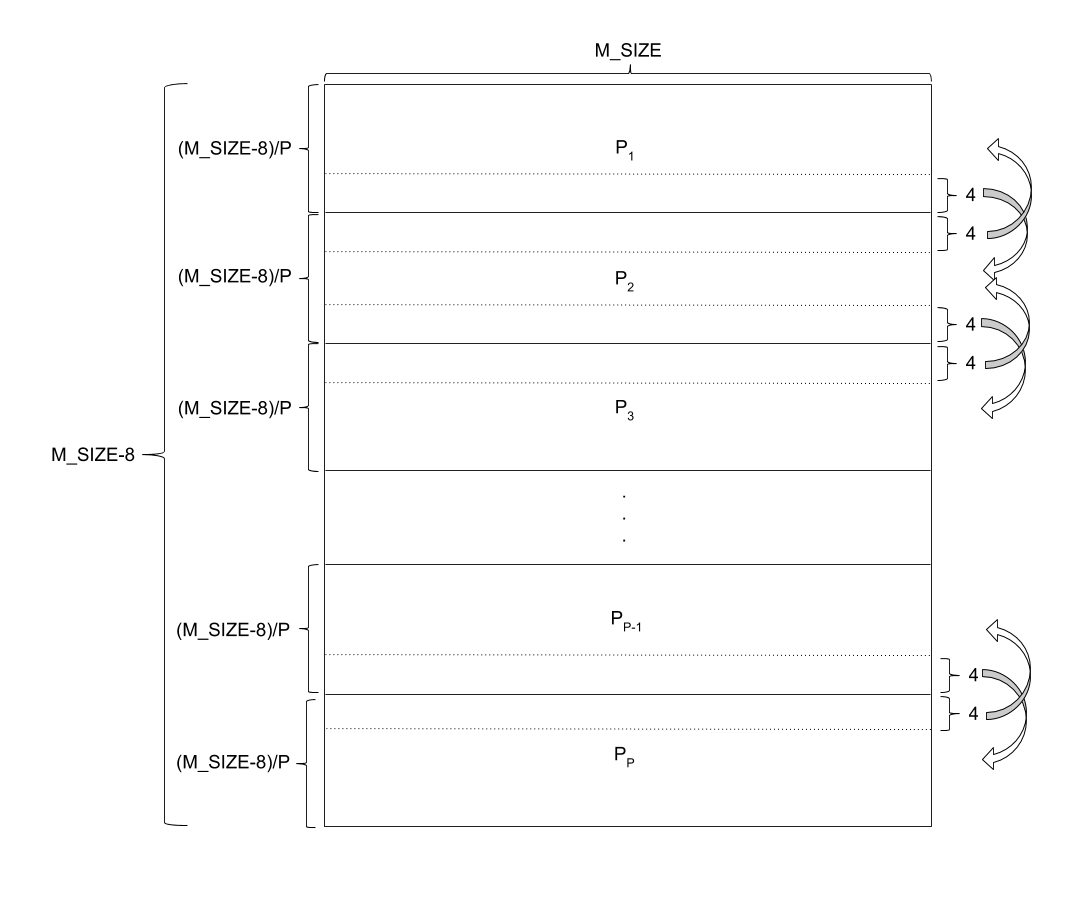
\includegraphics[width=15cm]{Pictures/matrixDraw.png}
\end{figure}


\section{Papel dos processos}
\label{procsMPI}
\begin{figure}[H]
    \centering
    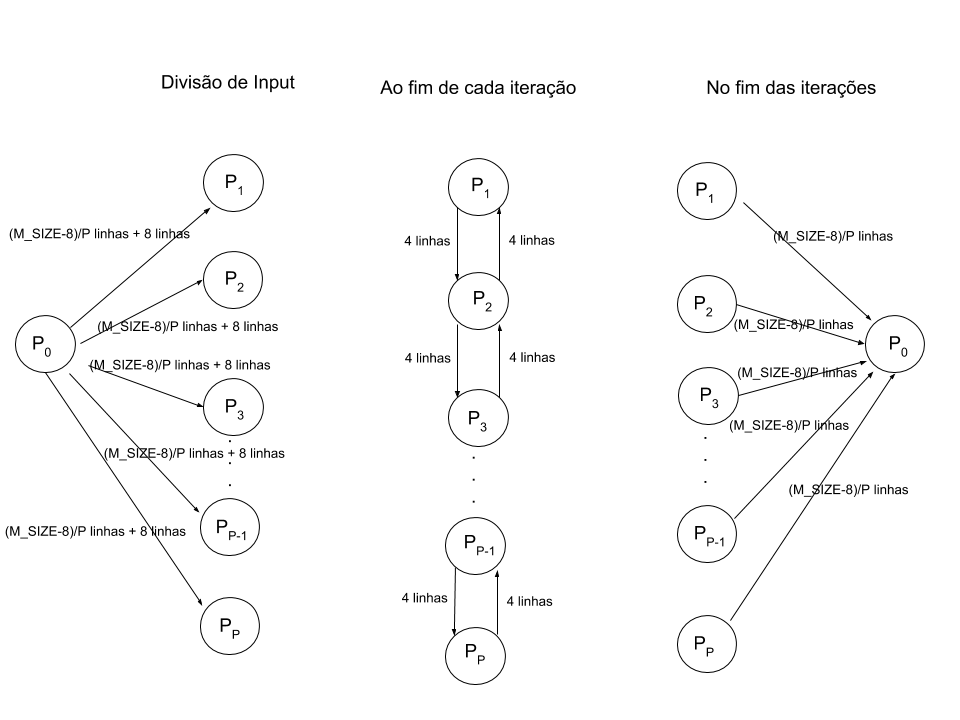
\includegraphics[width=15cm]{Pictures/graphDraw.png}
\end{figure}


\section{Análise Teórica-Fórmulas} \label{formulas}
\begin{equation}
T_{comp} = it*\frac{33*M^2}{P}*tc \label{eq:Tcomp}
\end{equation}

\begin{equation}
T_{comm} = 2*((M\_SIZE*M+M\_SIZE*4*P)*tw+ts*P) +  it*2*(ts+4*8*M\_SIZE*tw) \label{eq:Tcomm}
\end{equation}

\begin{equation}
T_{par} = it*\frac{33*M^2}{P}*tc + 2*((M\_SIZE*M+M\_SIZE*4*P)*tw+ts*P) +  it*2*(ts+4*8*M\_SIZE*tw) \label{eq:Tpar}
\end{equation}

\begin{equation}
T_{seq} = it*33*M^2*tc \label{eq:Tseq}
\end{equation}

\begin{equation}
G=\frac{it*33*M^2*tc}{it*\frac{33*M^2}{P}*tc + 2*((M\_SIZE*M+M\_SIZE*4*P)*tw+ts*P) + it*2*(ts+4*8*M\_SIZE*tw)} \label{eq:G}
\end{equation}

\section{MPI Communication Benchmark}
\label{pingpong_mpi}
\begin{verbatim}
double latency_test(MPI_Status status, int rank){
    double avg_time = 0.f;

    MPI_Barrier(MPI_COMM_WORLD);
    
    if(!rank)
        avg_time =  MPI_Wtime();
    for(int i = 0; i < SAMPLE_SIZE; i++){
        if(!rank){
            MPI_Send(NULL, 0, MPI_INT, 1, 1, MPI_COMM_WORLD);
            MPI_Recv(NULL, 0, MPI_INT, 1, 1, MPI_COMM_WORLD, &status);
        }else{
            MPI_Recv(NULL, 0, MPI_INT, 0, 1, MPI_COMM_WORLD, &status);
            MPI_Send(NULL, 0, MPI_INT, 0, 1, MPI_COMM_WORLD);
        }    
    }
    
    MPI_Barrier(MPI_COMM_WORLD);
    if(!rank)
        avg_time = MPI_Wtime() - avg_time;

    avg_time = avg_time/SAMPLE_SIZE*1.0e6;
    return avg_time/2;                          // half round trip
}

double throughput_test(double latency, MPI_Status status, int rank){
    double avg_time = 0.f;
    double *vec = (double*)calloc(VEC_SIZE, sizeof(double));
    
    MPI_Barrier(MPI_COMM_WORLD);

    if(!rank)
        avg_time = MPI_Wtime();
    for(int i = 0; i < SAMPLE_SIZE; i++){
        if(!rank){
            MPI_Send(vec, VEC_SIZE, MPI_DOUBLE, 1, 1, MPI_COMM_WORLD);
            MPI_Recv(vec, VEC_SIZE, MPI_DOUBLE, 1, 1, MPI_COMM_WORLD, &status);
        }else{
            MPI_Recv(vec, VEC_SIZE, MPI_DOUBLE, 0, 1, MPI_COMM_WORLD, &status);
            MPI_Send(vec, VEC_SIZE, MPI_DOUBLE, 0, 1, MPI_COMM_WORLD);
        }
    }

    MPI_Barrier(MPI_COMM_WORLD);

    if(!rank)
        avg_time = MPI_Wtime() - avg_time;
    avg_time = avg_time/SAMPLE_SIZE*1.0e6-2*latency;

    return avg_time/(2*VEC_SIZE*sizeof(double));
}

double computation_test(int rank){
    double avg_time=0.f;
    double *vec = (double*)malloc(VEC_SIZE*sizeof(double));
    double c[5];
    initiateMask(c);

    MPI_Barrier(MPI_COMM_WORLD);

    if(!rank)
        avg_time = MPI_Wtime();
    for(int i = 0; i < SAMPLE_SIZE; i++){
        vec[PIVOT] = vec[PIVOT]*c[0];
        for(int w = 1; w <= STENCIL_P; w ++)
            vec[PIVOT] += c[w]*vec[PIVOT+w] + c[w]*vec[PIVOT-w];
    }

    MPI_Barrier(MPI_COMM_WORLD);

    if(!rank)
        avg_time = MPI_Wtime() - avg_time;
    avg_time = avg_time/SAMPLE_SIZE*1.0e6;

    return avg_time/17;             //no. of ops: additions + multiplications
}
void fillArray(int array[], int arraySize) {
        int i;
        // use current time as seed for random generator
        srand(time(0));
        for (i = 0; i < arraySize; i++) {
                array[i] = rand() % 100; //INT_MAX
        }
}

void boolean_test(){
    int N = 1000000;
    double startTime, endTime;
    int x[N];
    int y[N];
    int i=0, b;

    fillArray(x,N);
    fillArray(y,N);

    //Start timing
    startTime = omp_get_wtime();

    while(i<N){
        b = (x[i] < y[i]);
        i++;
    }

    //End timing
    endTime = omp_get_wtime() - startTime;
    printf("%f\n", endTime);
}

int main(){
    boolean_test();
    return 0;
}
\end{verbatim}

\section{Speed-up Teórico}
\begin{figure}[H]
    \centering
    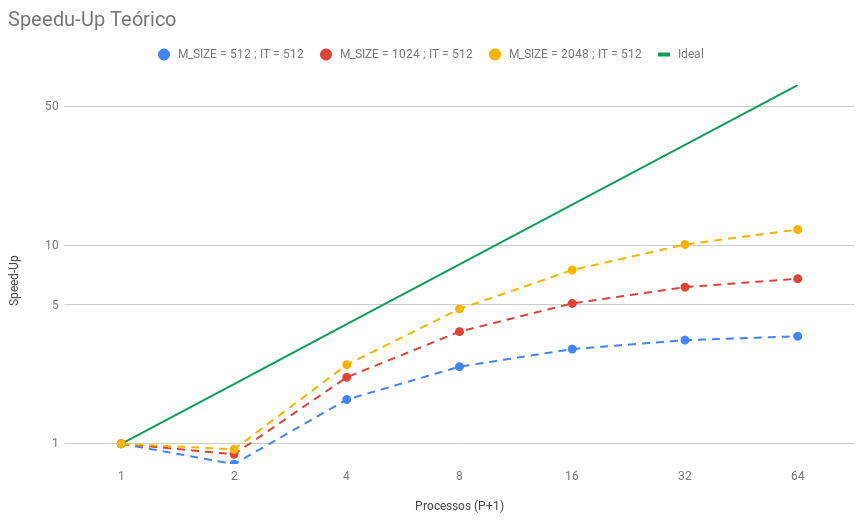
\includegraphics[width=15cm]{Pictures/TheoreticalGraph1.png}
    \caption{Speed-up teórico do Stencil}
    \label{theoretical_stencil}
\end{figure}

\begin{figure}[H]
    \centering
    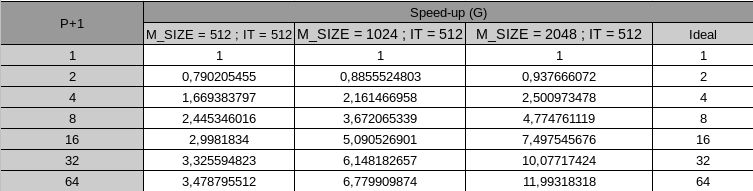
\includegraphics[width=15cm]{Pictures/TheoreticalTbl1.png}
    \caption{Speed-up teórico do Stencil}
\end{figure}

\begin{figure}[H]
    \centering
    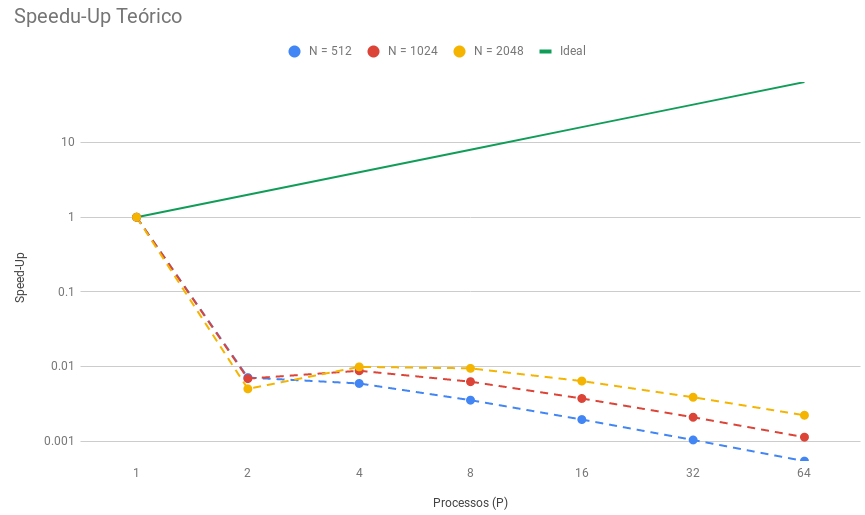
\includegraphics[width=15cm]{Pictures/TheoreticalGraph2.png}
    \caption{Speed-up teórico do Merge Sort}
    \label{theoretical_mergeSort}
\end{figure}

\begin{figure}[H]
    \centering
    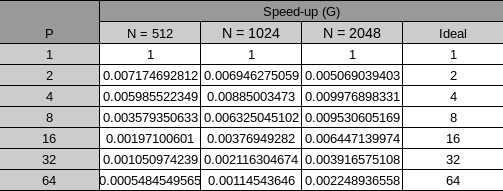
\includegraphics[width=15cm]{Pictures/TheoreticalTbl2.png}
    \caption{Speed-up teórico do Merge Sort}
\end{figure}

\section{Resultados Experimentais}

\begin{figure}[H]
    \centering
    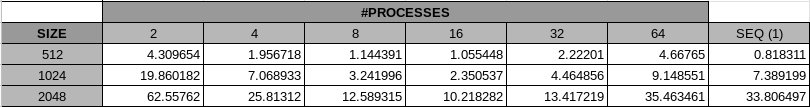
\includegraphics[width=19cm]{Pictures/ExperimentalTable1.png}
    \caption{Medianas dos Tempos do Stencil}
    \label{resStencil}
\end{figure}

\begin{figure}[H]
    \centering
    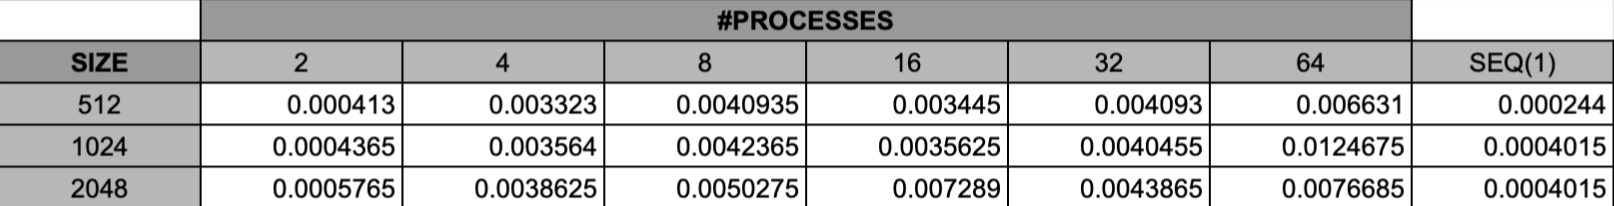
\includegraphics[width=19cm]{Pictures/ExperimentalTable2.png}
    \caption{Medianas dos Tempos do Merge Sort}
    \label{resMergeSort}
\end{figure}

\section{Tempo de Comunicação}

\begin{figure}[H]
    \centering
    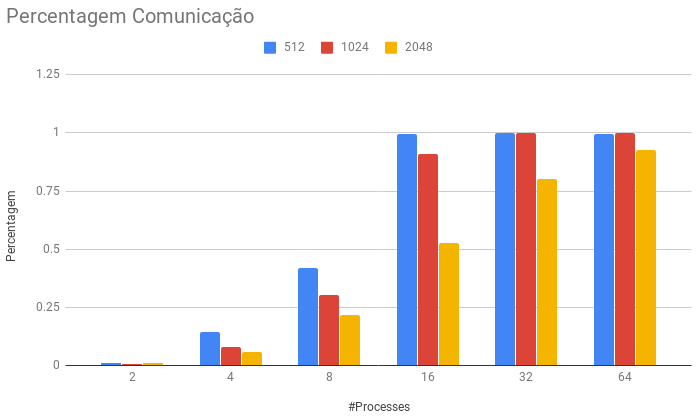
\includegraphics[width=17cm]{Pictures/comm_temp1.png}
    \caption{Percentagem de tempo atribuído a comunicação do Stencil}
    \label{tempStencil}
\end{figure}

\begin{figure}[H]
    \centering
    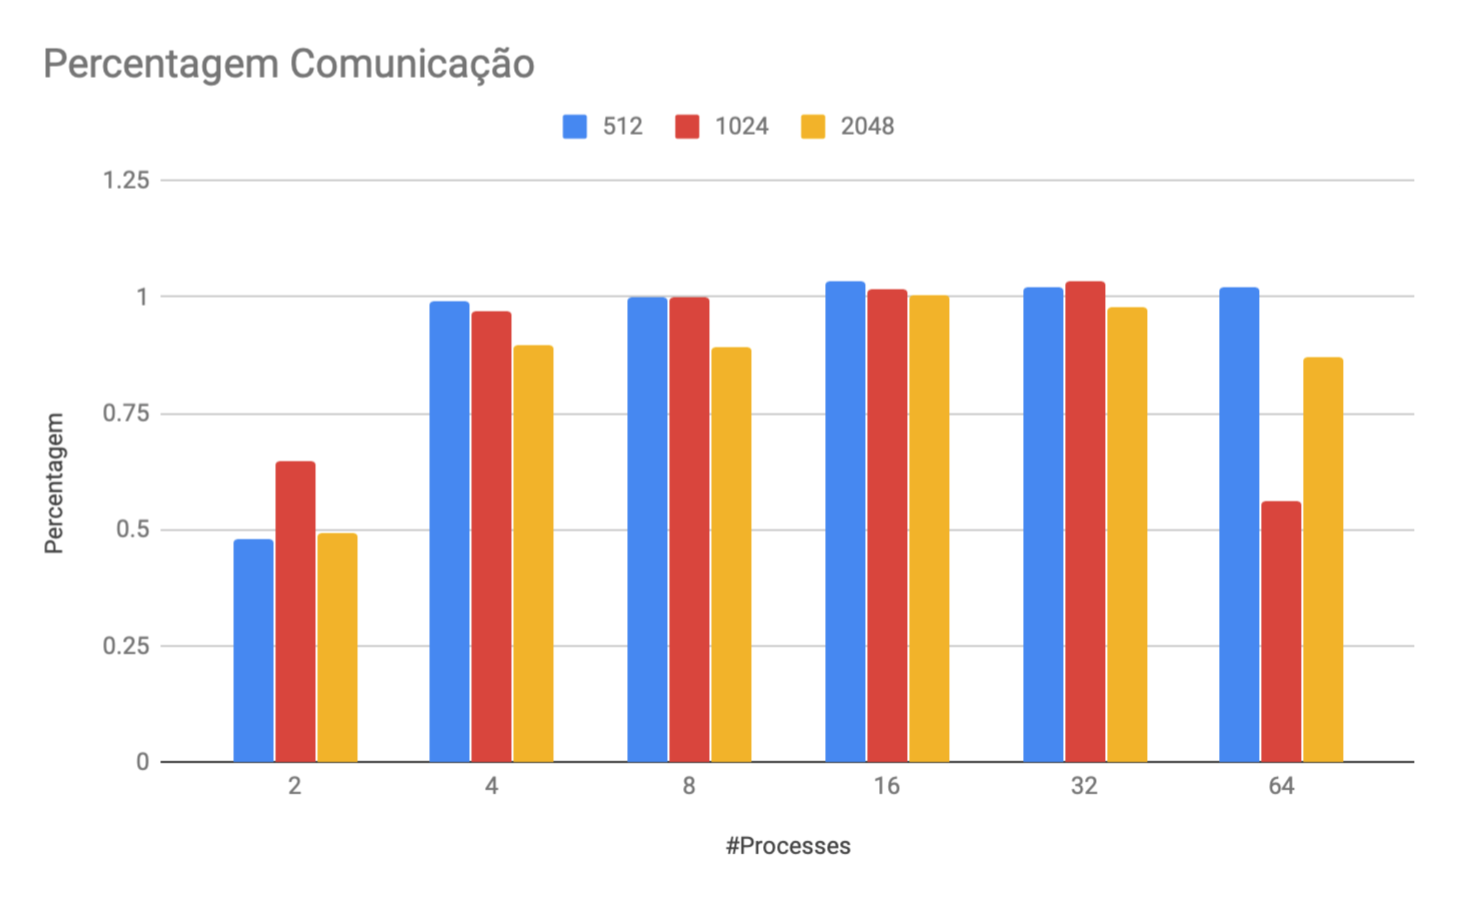
\includegraphics[width=17cm]{Pictures/comm_temp2.png}
    \caption{Percentagem de tempo atribuído a comunicação do Merge Sort}
    \label{tempMergeSort}
\end{figure}

\section{Speed-up MPI Experimental}
\begin{figure}[H]
    \centering
    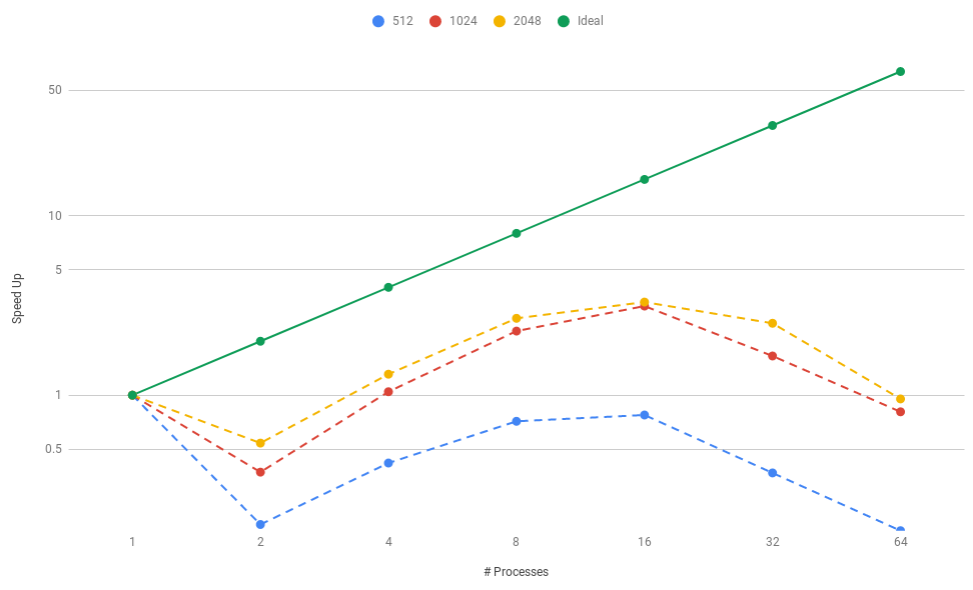
\includegraphics[width=16cm]{Pictures/ExperimentalGraph1.png}
    \caption{Speed-up experimental MPI do Stencil}
    \label{graphStencil}
\end{figure}

\begin{figure}[H]
    \centering
    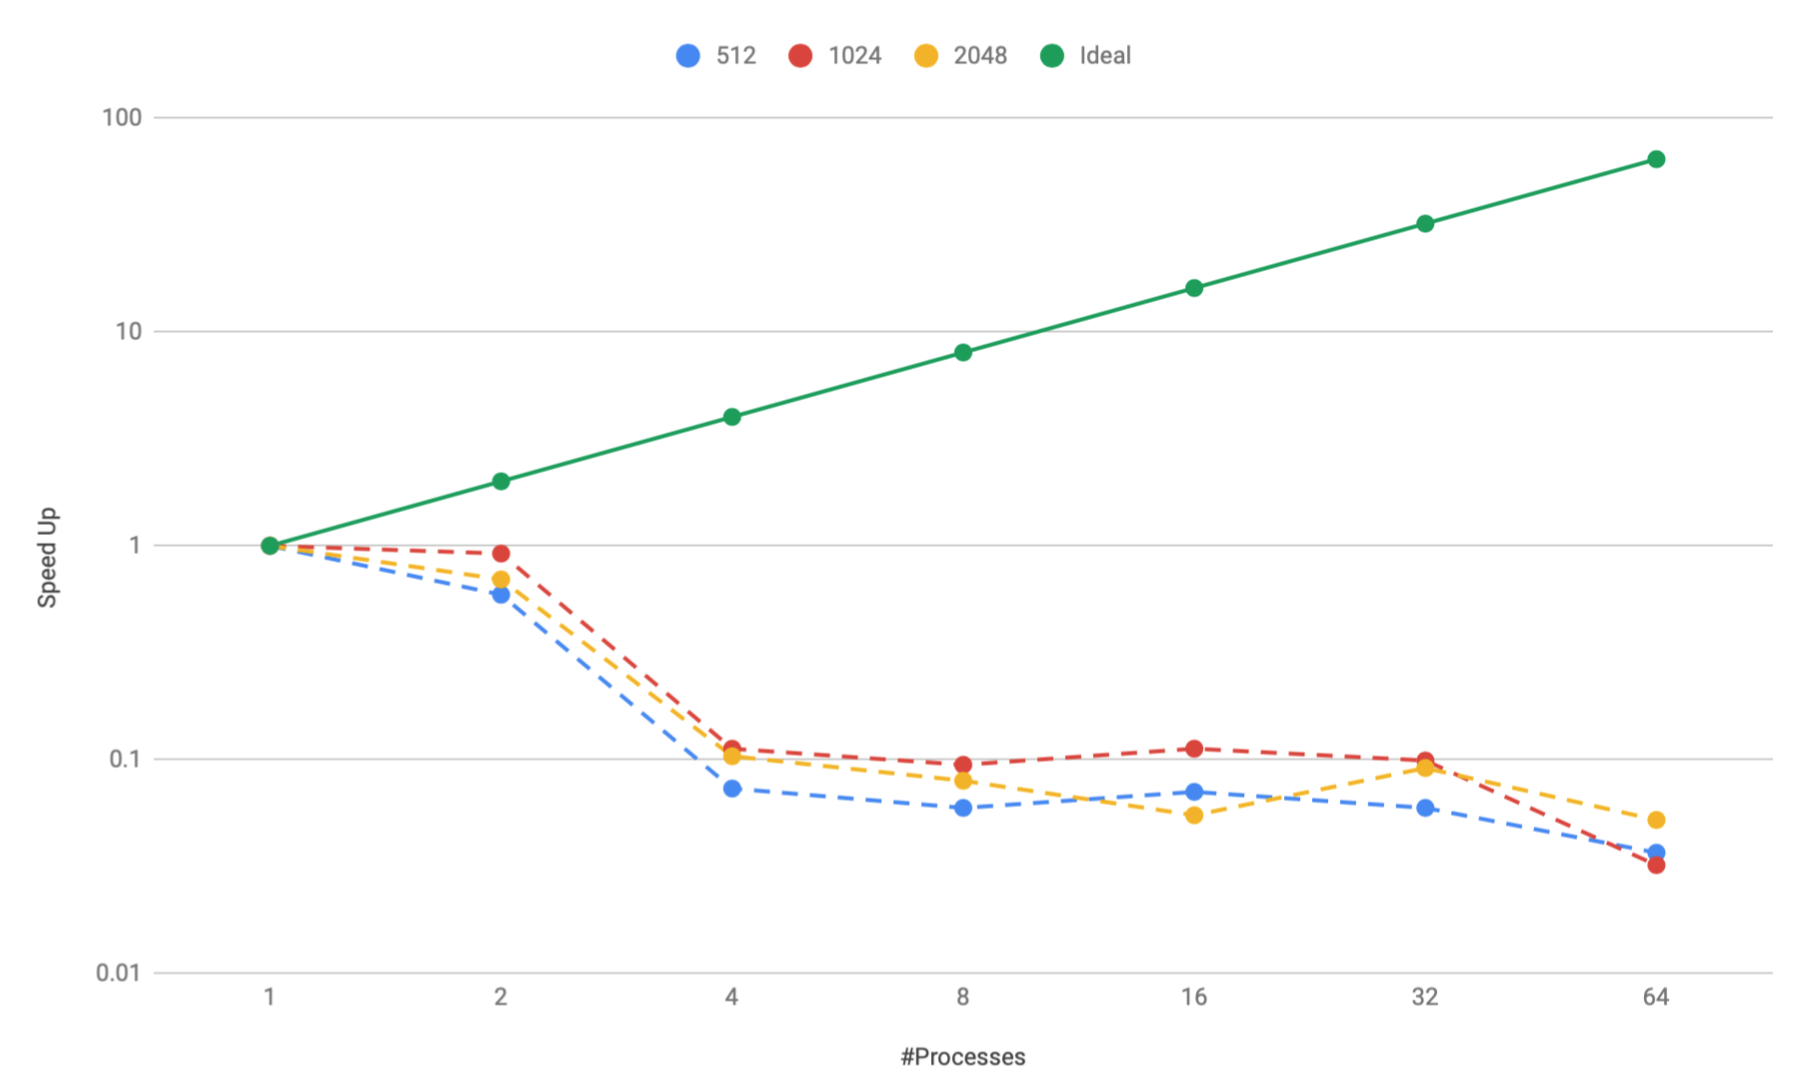
\includegraphics[width=16cm]{Pictures/ExperimentalGraph2.png}
    \caption{Speed-up experimental MPI do Merge Sort}
        \label{graphMergeSort}
\end{figure}

\section{Contexto de experimentação}

\label{lab_config}
\begin{tabular}{|c|c|c|c|}
\hline
\textbf{Ordem(N)} & \textbf{Nro. de processos} & \textbf{Mapeamento de processos} & \textbf{Nro. de nodos} r641 \\
\hline
N=512           & 2, 4, 8, 16, 32, 64  & \texttt{--map-by} node & 2 \\
\hline
N=1024          & 2, 4, 8, 16, 32, 64  & \texttt{--map-by} node & 2 \\
\hline
N=2048          & 2, 4, 8, 16, 32, 64  & \texttt{--map-by} node & 2 \\
\hline
\end{tabular}
\end{appendix}

\end{document}
